\documentclass[a4paper, 10pt]{article}
    \usepackage[utf8]{inputenc}
    \usepackage{fullpage}
    \usepackage{enumitem}
    \usepackage{graphicx}
    \graphicspath{{images/}}
    \usepackage[urlcolor=blue]{hyperref}

    % No indent on new paragraph
    \setlength{\parindent}{0em}

    \setlength{\parskip}{1em}
    \renewcommand{\baselinestretch}{1.15}

    \title{COP 5615 - Project 2 Report}
    \author{Vaibhav Yenamandra ($1931$-$4050$)\\ email: \href{vyenaman@ufl.edu}{vyenaman@ufl.edu} }
    \date{\today}

    \begin{document}

    \maketitle

    \section{Gossip}

    \begin{figure}[h]
      \caption{Gossip Convergence Time v/s Network size}
      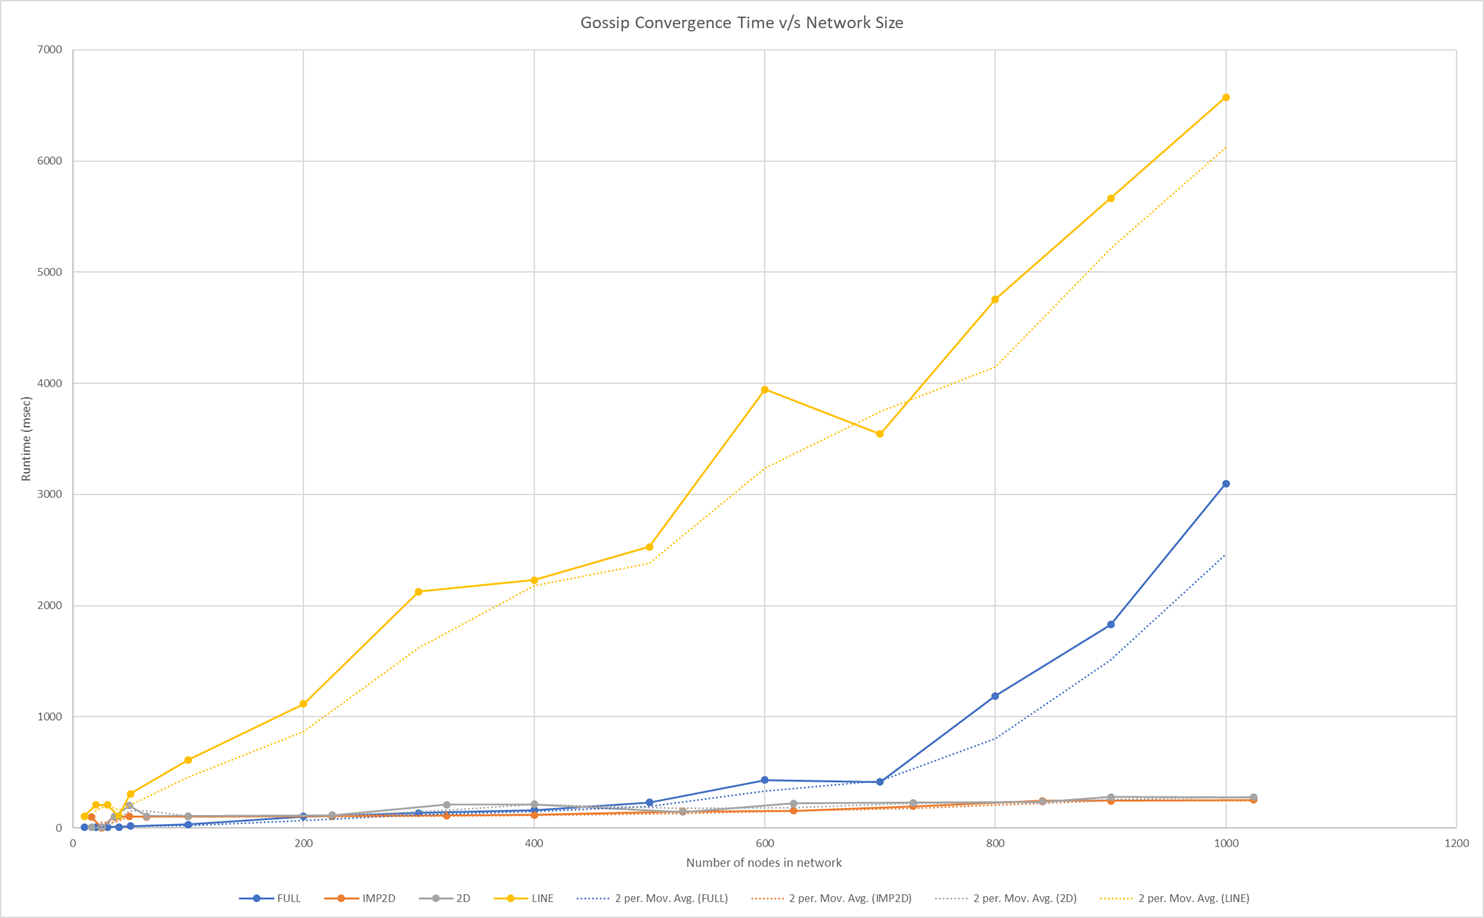
\includegraphics[width=\textwidth]{project2_gossip_chart}
    \end{figure}

    Covergence rates from the data extracted resemble the following:
    \begin{enumerate}
      \item{Line: $O(n)$}
      \item{Full: $O(n^2)$}
      \item{2D Grid: $O(\log n)$}
      \item{Imperfect 2D Grid: $O(\log n)$}
    \end{enumerate}

    The above figure shows the convergence times of various network topologies (see legend) vs the number of nodes in the network. For the project I defined convergence as the following routine:
    \begin{enumerate}
      \item{Check if more than $50\%$ of network is in a terminated state, if yes, return \texttt{true}, if not, go to the next step}
      \item{Check if less than $1\%$ of the network has not heard the rumour yet, if yes, return \texttt{true}, else return \texttt{false}}
    \end{enumerate}

    \section{Push-sum}
    \begin{figure}[h]
      \caption{Push-sum Convergence Time v/s Network size}
      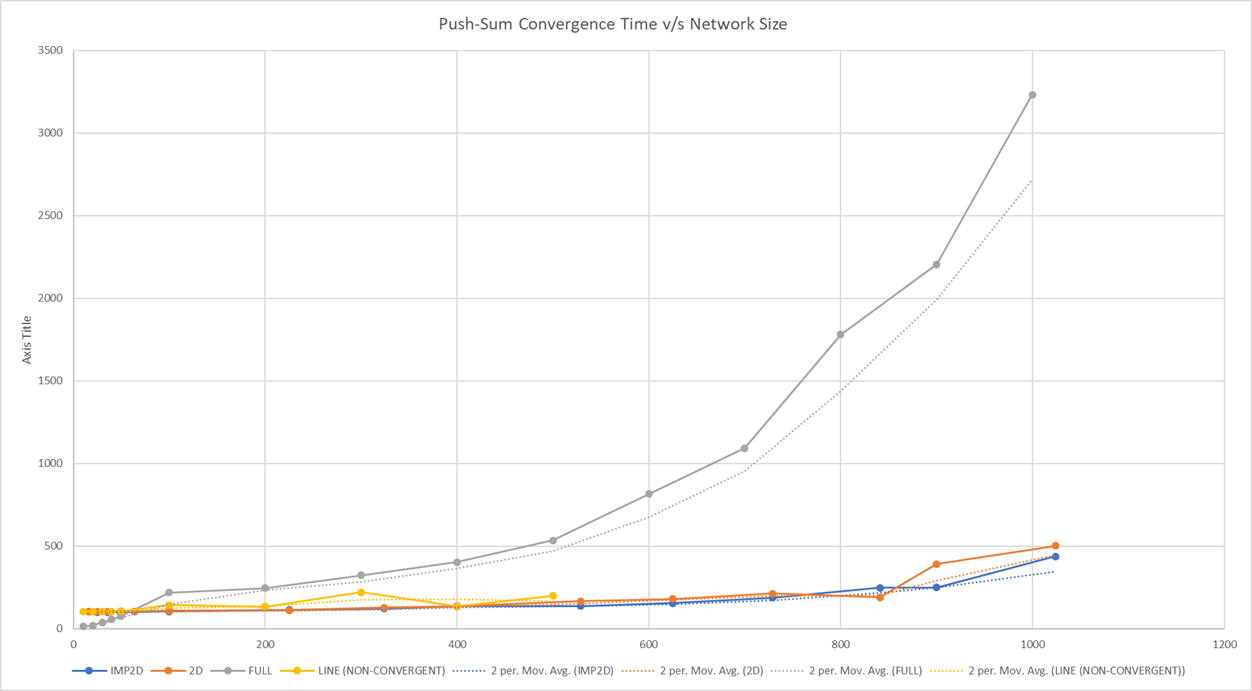
\includegraphics[width=\textwidth]{project2_psum_chart}
    \end{figure}

    Covergence rates from the data extracted resemble the following. Note that data for line is not clean since it doesn't actually converge to any correct value, and results in more timeouts than actual results.
    \begin{enumerate}
      \item{Line: $O(n)$}
      \item{Full: $O(n^2)$}
      \item{2D Grid: $O(\log n)$}
      \item{Imperfect 2D Grid: $O(\log n)$}
    \end{enumerate}

    To check if the push sum network has converged we check if more than $50\%$ of the network has reached a stable value.

\end{document}
